\usetikzlibrary{shapes.geometric, arrows}

% Style for process block.
\tikzstyle{process} = [rectangle, text width=2.5cm, minimum width=2.5cm, minimum height=1.5cm,text centered, draw=black,
fill=orange!30]

% Style for terminal block.
\tikzstyle{terminal} = [rectangle, text width=2cm, minimum width=2cm, minimum height=1.5cm,text centered,
draw=black, fill=red!30]

% Style for decision block.
\tikzstyle{decision} = [diamond, text width=1.5cm, minimum width=2.5cm, minimum height=2.5cm,text centered, draw=black,
fill=green!30, inner sep=-12pt]

% Style for line.
\tikzstyle{line} = [draw, -latex']

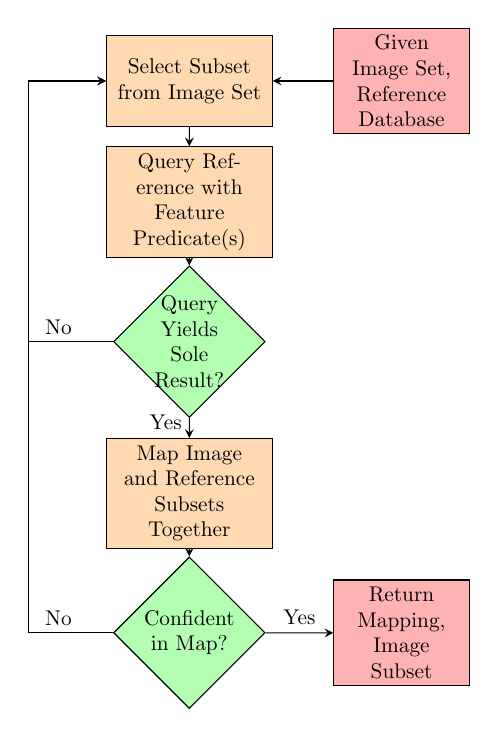
\begin{tikzpicture}[node distance=1.3cm, scale=0.77, transform shape]
    \node[scale=1](getImage)[terminal]{Given Image Set, Reference Database};
    \node[scale=1](pickQueryStars) [process, left of=getImage, xshift =-2.2cm] {Select Subset from Image Set};
    \node[scale=1](searchCatalog)[process, below of=pickQueryStars, yshift=-0.7cm] {Query Reference with Feature Predicate(s)};
    \node[scale=1](confidentInCatalog)[decision, below of=searchCatalog, yshift=-1cm] {Query Yields Sole Result?};
%    \node[scale=1](filterCandidates)[process, below of=confidentInCatalog, yshift=-0.4cm] {Select Candidate $R[1]$};
%    \node[scale=1](confidentAfterFilter)[decision, below of=filterCandidates, yshift=-0.4cm] {Confident?};
    \node[scale=1](findMap)[process, below of=confidentInCatalog, yshift=-1.2cm]{Map Image and Reference Subsets Together};
    \node[scale=1](confidentInMap)[decision, below of=findMap, yshift=-1cm] {Confident in Map?};
    \node[scale=1](returnMap)[terminal, right of=confidentInMap, xshift = 2.2cm] {Return Mapping, Image Subset};

    \draw[->,>=stealth](getImage.west) -- (pickQueryStars.east);
    \draw[->,>=stealth] (pickQueryStars) -- (searchCatalog);
    \draw[->, >=stealth] (searchCatalog) -- (confidentInCatalog);
    \draw[->,>=stealth] (confidentInCatalog) -- node[anchor=east, yshift=0.1cm]{Yes}(findMap);
%    \draw[->, >=stealth] (confidentInCatalog) -- node[anchor=east, yshift=0.1cm]{Yes}(filterCandidates);
%    \draw[->, >=stealth] (filterCandidates) -- (findMap);
%    \draw[->, >=stealth] (confidentAfterFilter) -- node[anchor=east, yshift=0.1cm]{Yes} (findMap);
    \draw[->, >=stealth] (findMap) -- (confidentInMap);
    \draw[->, >=stealth] (confidentInMap) -- node[xshift=0cm, yshift=0.25cm]{Yes} (returnMap);

    \draw[->, >=stealth] (confidentInCatalog.west) -- ++(-1.4cm, 0cm) node[anchor=south, xshift=0.5cm]{No}
    |- (pickQueryStars.west);
%    \draw[->, >=stealth] (confidentAfterFilter.west) -- ++(-1.4cm, 0cm) node[anchor=south, xshift=0.5cm]{No}
%    |- (pickQueryStars.west);
    \draw[->, >=stealth] (confidentInMap.west) -- ++(-1.4cm, 0cm) node[anchor=south, xshift=0.5cm]{No}
    |- (pickQueryStars.west);
\end{tikzpicture}